\chapter{El transistor}\label{chapter:transistor}

Antes de la invención del primer transistor a finales de la década de 1930, ya existían dispositivos que cumplían la misma función que 
este pero con una menor eficiencia.\\
\indent A finales del siglo XIX con el incipiente desarrollo de la tecnología de comunicación inalámbrica y la construcción de sistemas
que utilizaran este método por la \emph{compañía Marconi}, \emph{Guglielmo Marconi} le asignó el cargo de consejero científico al físico
inglés \emph{John Ambrose Fleming}. \emph{Marconi} necesitaba ayuda para mejorar el \textbf{detector}, que es el dispositivo que se
encarga de extraer información de una corriente de radiofrecuencia modulada, y aunque ya él había desarrollado un \textbf{detector
magnético}, este solo brindaba una señal de frecuencia de audio a un receptor de teléfono. Un \textbf{detector} confiable que pudiera
guiar un instrumento de impresión era necesario. Fleming pudo desarrollar un \textbf{tubo al vacío} como resultado de su trabajo con
\textbf{bombillas de efecto Edison}, a estas las denominó \textbf{válvulas de oscilación} ya que pasaba corriente en una sola dirección.
Fleming presentó una patente para estos tubos, cedida a la \emph{compañía Marconi} en el Reino Unido en noviembre de 1904 y esta se emitió
en septiembre de 1905. Conocida más tarde como la \textbf{válvula Fleming}, la \textbf{válvula de oscilación} se desarrolló con el fin de
rectificar la corriente de radiofrecuencia como componente detector de circuitos receptores de radio. \brackcite{wikipedia_2022_tube}\\
\indent En el propio siglo XIX ingenieros de telégrafos y teléfono habían reconocido la necesidad de incrementar la distancia que la señal
pudiera ser transmitida. En 1906 \emph{Robert Von Lieben} solicitó una patente para un \textbf{tubo de rayos catódicos} que usaba una bobina
de deflexión magnética externa y estaba destinado a usarse como amplificador en equipos de telefonía. A \emph{Lee de Forest} se le acredita
la invención del tubo triodo en 1907, el cual tenía la capacidad de amplificar las señales, y que fue el primero de su tipo que tuvo uso
práctico. Sin embargo estos \textbf{tubos de vacío} utilizados para amplificar la música y la voz que hicieron posibles las llamadas de
larga distancia, creaban mucho calor y se quemaban muy rápido, requiriendo alto mantenimiento. \brackcite{wikipedia_2022_tube, wikipedia_2022_triode}\\
\indent La \textbf{ENIAC}(\emph{Electronic Numerical Integrator and Computer}) fue la primera computadora en usar los \textbf{tubos de vacío},
exactamente 18 000 de estos para poder funcionar, que hicieron que aquel dispositivo ocupara el tamaño de una habitación completa. Estos tubos
permitían que las señales fueran enviadas y los cálculos realizados de forma más rápida a través del uso de conmutación eléctrica en vez de
conmutación mecánica. Debido al enorme consumo de energía eléctrica de la \textbf{ENIAC}, muchas personas creyeron que esta se destruiría,
sin embargo los \textbf {tubos de vacío} le permitieron soportar y funcionar. ~\brackcite{richards_2022}.\\

\begin{figure}[htb]
	\centering
	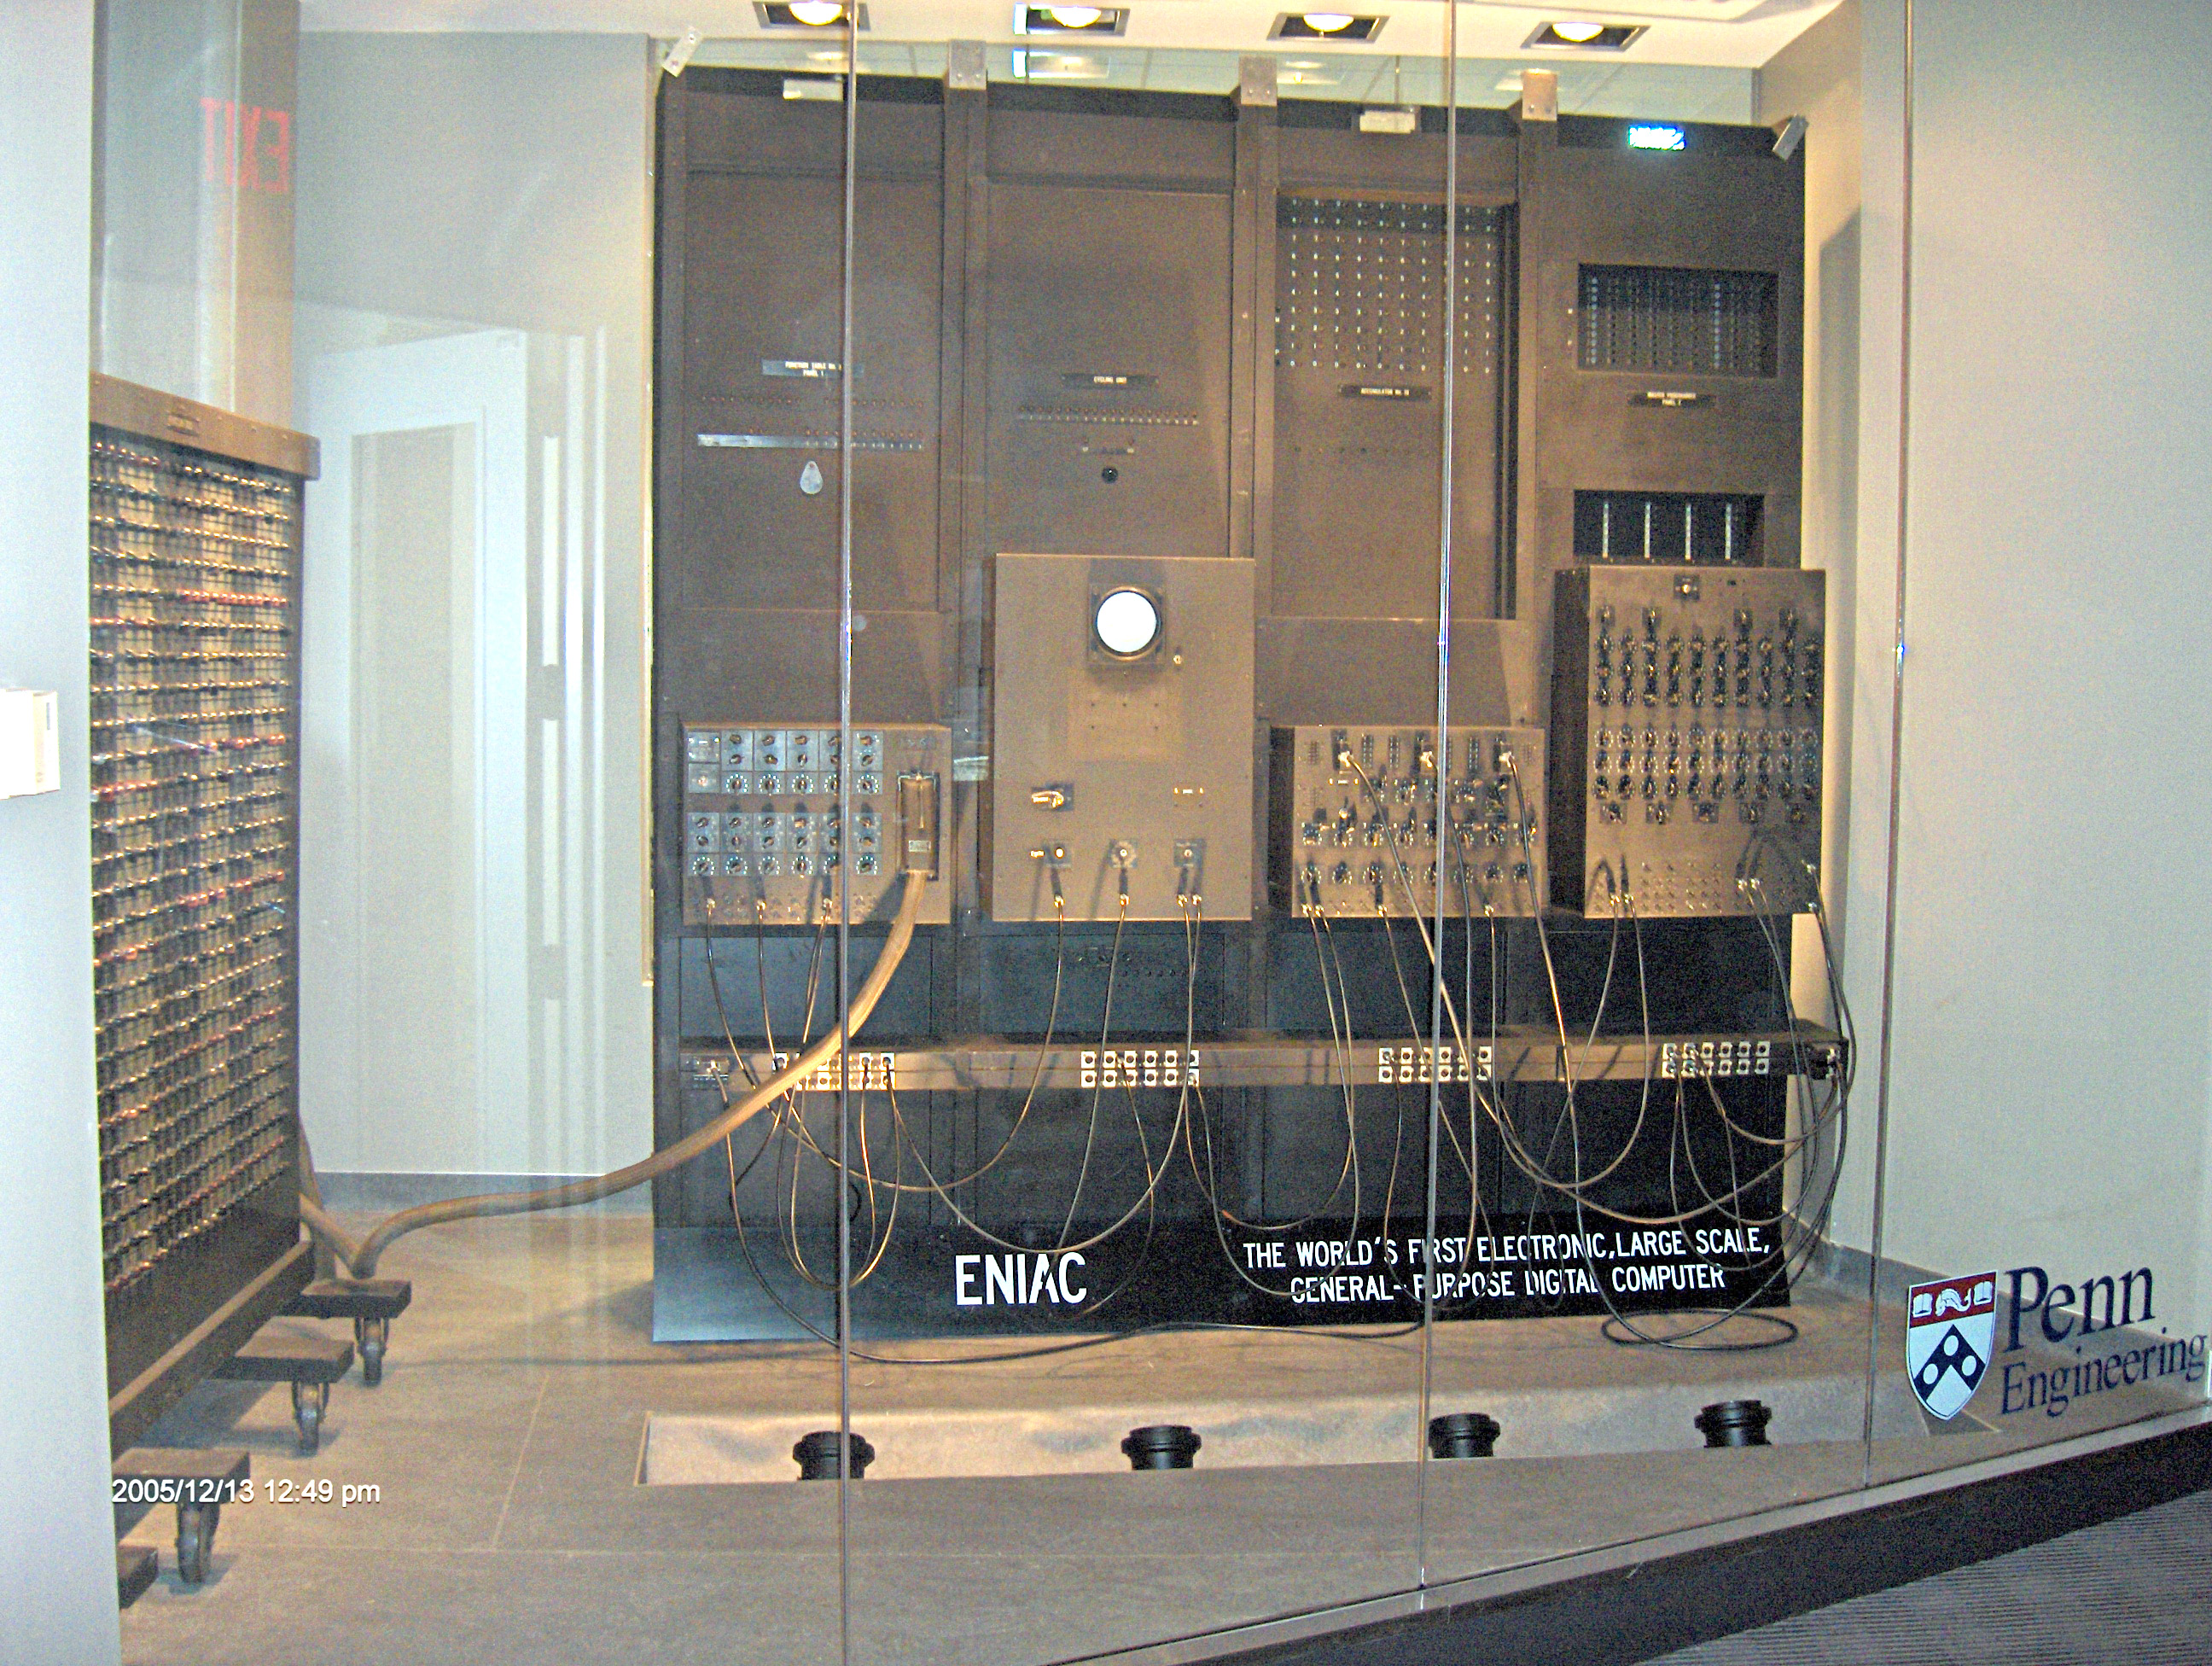
\includegraphics[scale = 0.13]{Graphics/ENIAC.jpg}
	\caption{\textbf{ENIAC} primera computadora que utilizó los \textbf{tubos de vacío}.}
	\label{fig:1}
\end{figure}

\section{El surgimiento}
Debido a que las computadoras dependían de los \textbf{tubos de vacío} tan frágiles, grandes,
costosos y con un consumo enorme de energía, solo las grandes compañías, los militares y las
universidades con proyectos de investigación podían permitírselas. Por esta razón el inicio de la
era digital, aquella donde los dispositivos electrónicos se convertirían en una parte indispensable
en nuestro día a día, no ocurriría sino hasta el martes 16 de diciembre de 1947. Ese día 2 científicos
en los \emph{laboratorios Bell} lograron armar un pequeño artilugio que habían inventado a partir de
unas tiras de oro, papel de aluminio, un trozo de material semiconductor(\textbf{germanio}) y un sujetapapeles
doblado, el cual movido a la perfección podía amplificar una corriente eléctrica y encenderla y apagarla.\\
Durante mucho tiempo hubo una persona encargada de encontrar un reemplazo para los \textbf{tubos 
de vacío}, un reemplazo menos costoso, más sólido y más barato, esa persona fue el físico experto
en estado sólido \emph{William Shockley}, graduado del \textbf{MIT}(\emph{Massachussets Institute of Technology}),
quien fue contratado por \emph{Mervin Kelly} jefe del departamente de \textbf{tubos al vacío} de los \emph{
labotorios Bell} con este fin. Luego de 3 años a \emph{Shockley} se le ocurrió que podría encontrar una
solución utilizando materiales sólidos como el \textbf{silicio} en vez de los filamentos de una bombilla, “Se 
me ha ocurrido que es posible crear un amplificador utilizando semiconductores en vez del vacío",
escribió \emph{Shockley}. Él parecía tener la capacidad de visualizar la teoría cuántica por cómo explicaba
el movimiento de los electrones. Sus colegas decían que podía mirar material semiconductor y ver los
electrones. Sin embargo, para transformar su intuición en un invento real, \emph{Shockley} necesitaba
un socio que fuera un hábil experimentador, y fue \emph{Walter Brattain} quien disfrutaba creando
dispositivos con semiconductores quien se unió a \emph{Shockley} en su tarea. Lamentablemente sus
ideas tuvieron que esperar pues recién comenzó la II Guerra Mundial, y no fue hasta casi 4 años
después que regresaron a su trabajo en los laboratorios que retomaron su investigación, y fueron
asignados a un grupo cuyo objetivo principal era encontrar el tan buscado reemplazo sólido para
los \textbf{tubos de vacío} utilizando semiconductores. Esta vez decidieron incorporar al grupo un 
nuevo teórico además de \emph{Shockley}, experto en teoría cuántica, \emph{John Bardeen}, un niño
genio que se había saltado tres grados en la escuela, \emph{Bardeen } había trabajado durante su servicio
en tiempos de guerra en la Artillería Naval y discutió el diseño de torpedos con nada más ni nada menos que 
\emph{Albert Einstein}. Él era uno de los mejores expertos del mundo en el uso de la teoría cuántica
para comprender cómo materiales conducen la electricidad, y tenía, según sus colegas, una “capacidad genuina
para colaborar fácilmente con experimentadores y teóricos". Así, ya se habían juntados los 3 hombres más importantes
de este proyecto. \brackcite{isaacson_2014}\\
\newpage

\begin{figure}[htb]
	\centering
	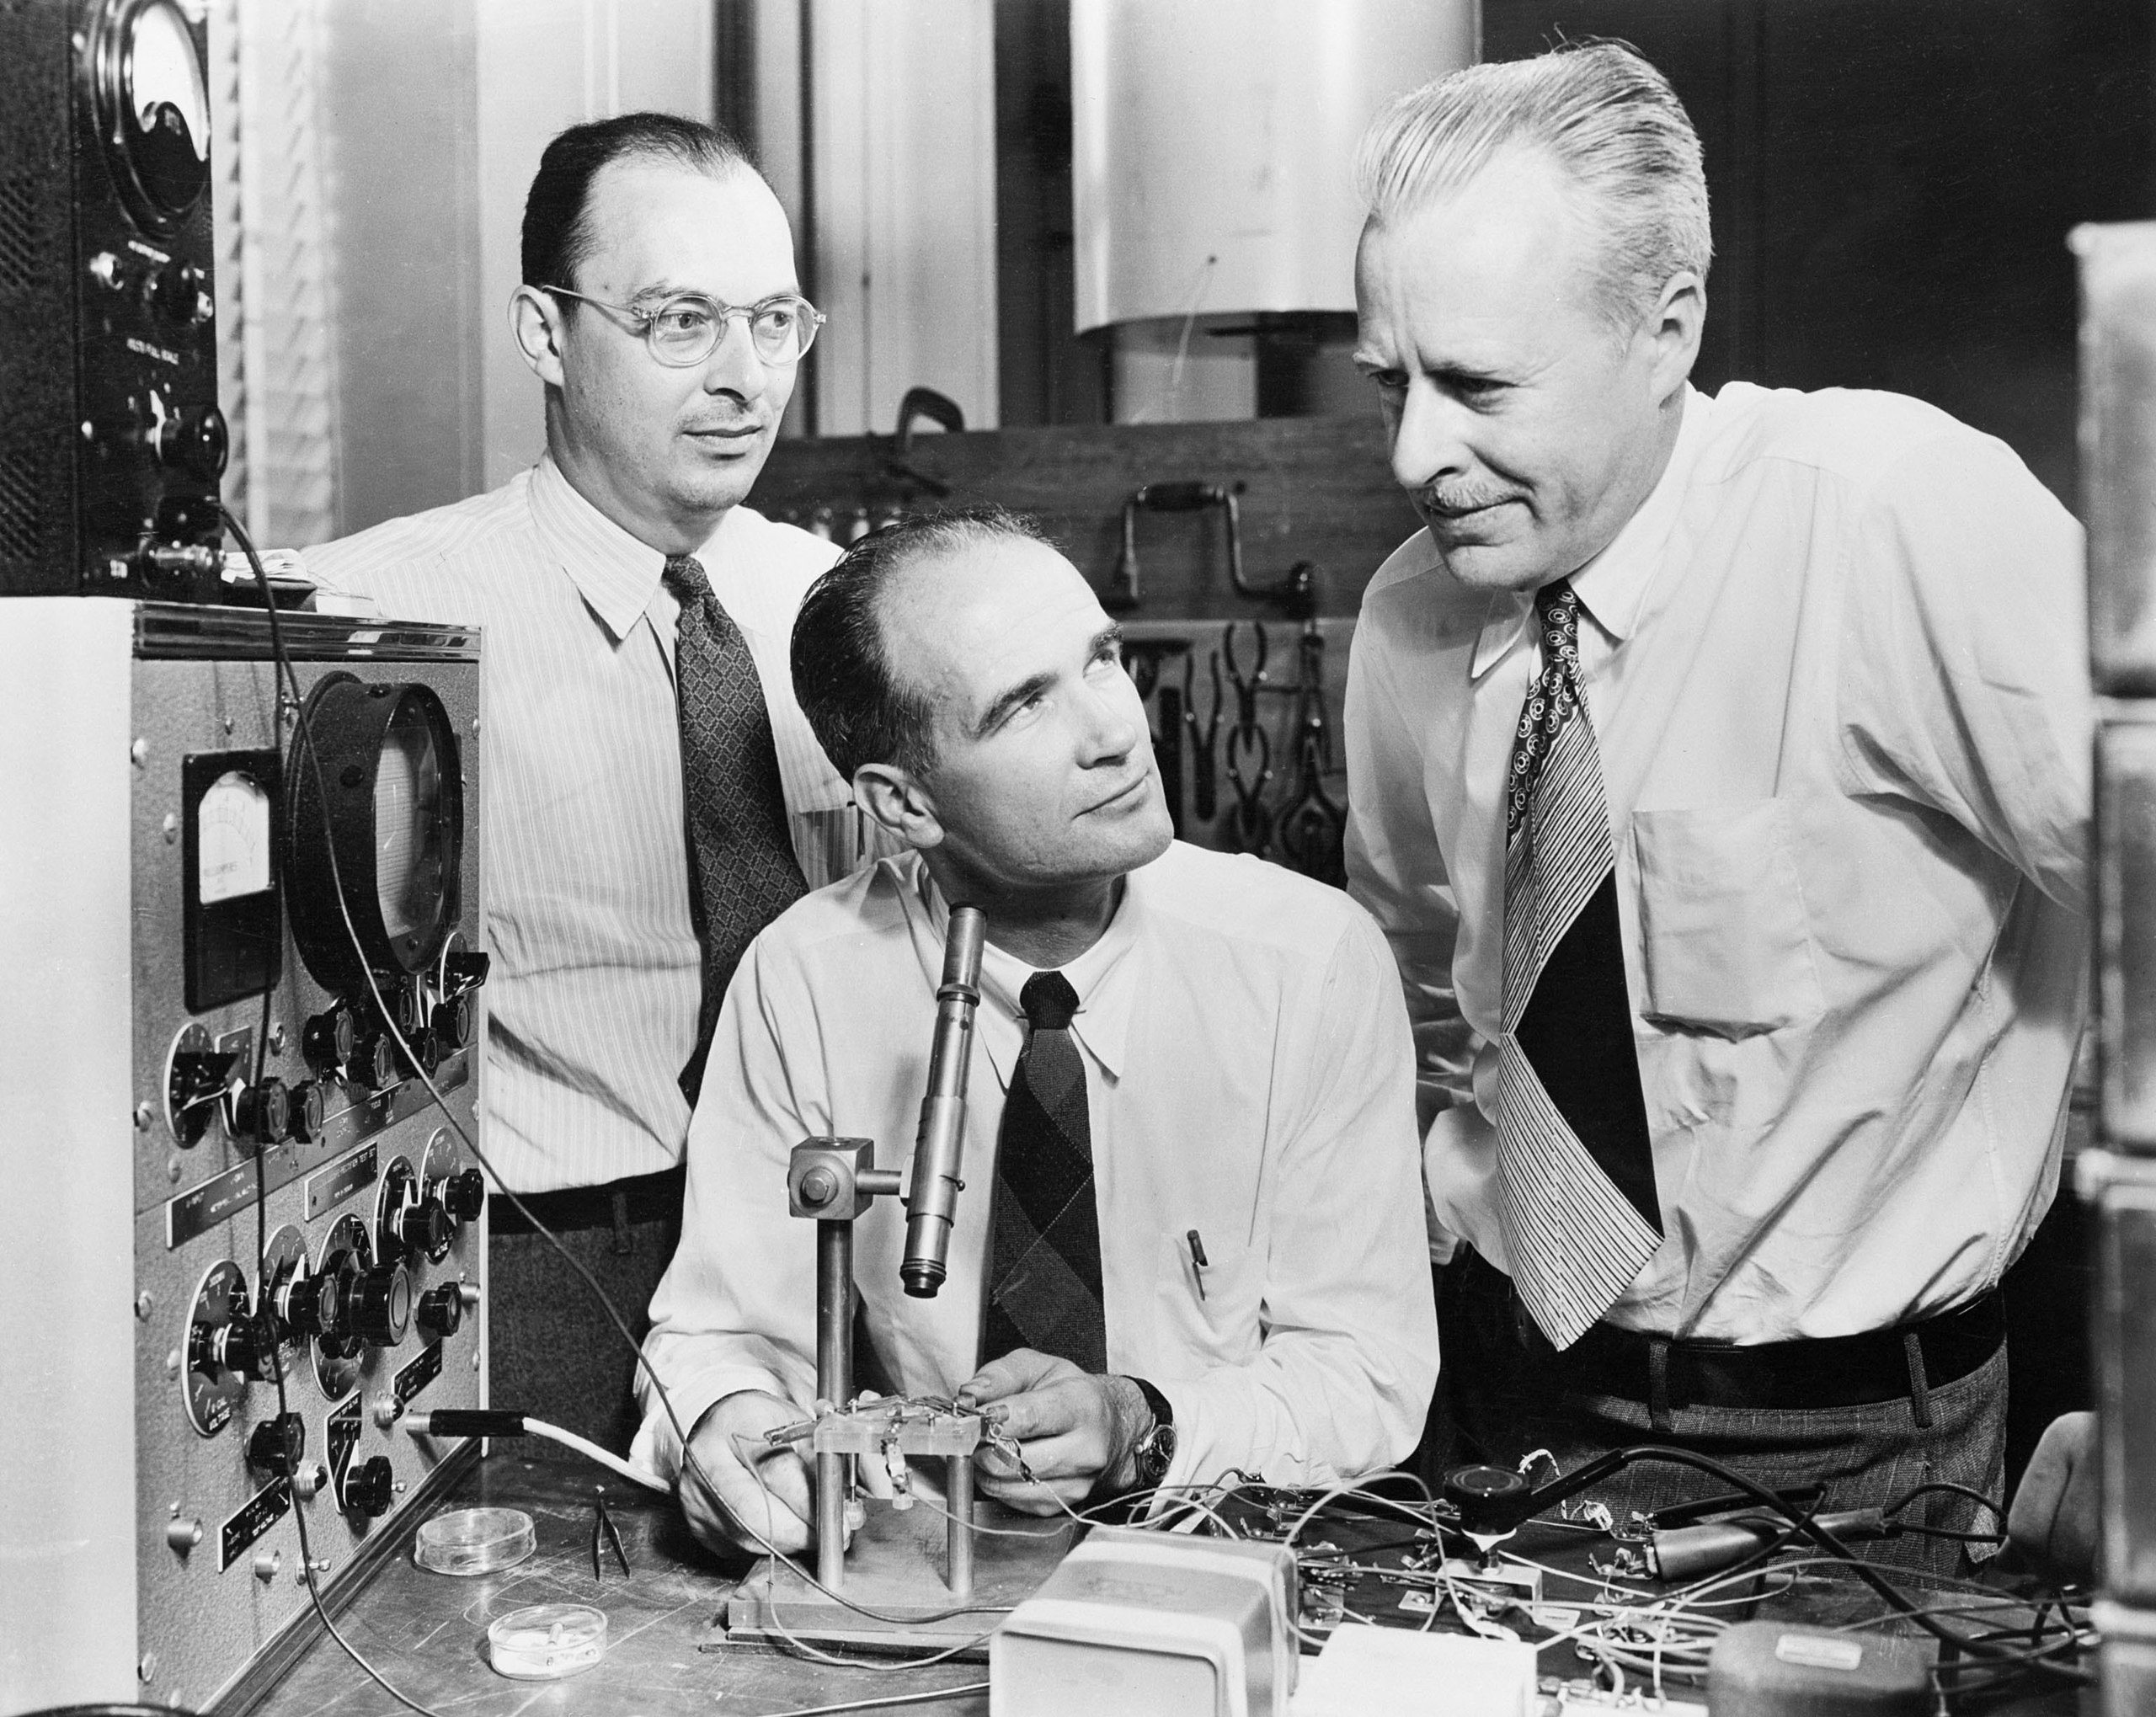
\includegraphics[scale = 0.13]{Graphics/Bardeen_Shockley_Brattain_1948.jpg}
\caption{\emph{John Bardeen, William Shockley} y \emph{Walter Brattain}, de izquierda a derecha en 1948.}
	\label{fig:2}
\end{figure}

Las más sorprendentes ideas provinieron de las interacciones entre ellos. "La cercana y constante colaboración entre
experimentalistas y teóricos se extendió a través de todas las etapas de la investigación, desde la concepción del
experimento hasta los análisis de los resultados”, dijo \emph{Bardeen}. Gracias a esta estrecha colaboración fue que 
el 16 de diciembre de 1947 lograron crear el primer \textbf{transistor} de la historia.\\

\begin{figure}[htb]
	\centering
	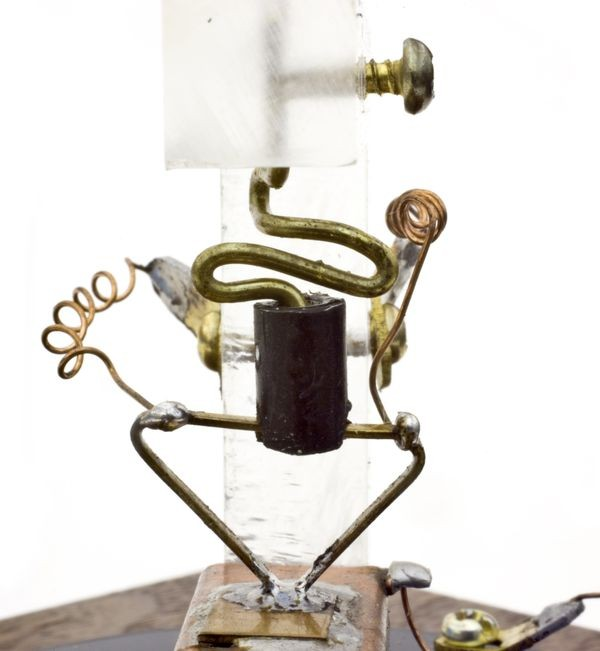
\includegraphics[scale = 0.2]{Graphics/first_transistor_replica.jpg}
	\caption{Réplica del primer \textbf{transistor}.}
	\label{fig:3}
\end{figure}

Los \emph{laboratorios Bell} fueron el fruto de un inmenso trabajo y hasta cierto punto una apuesta de la \textbf{AT\&T}
(\emph{American Telephone and Telegraph Company}) que a principios de 1907 pasaba por una grave crisis, y con la guía
\emph{Alexander Graham Bell}, \emph{Theodore Vail} y el apoyo de la junta directiva lograron salvar a la empresa de la quiebra,
y a la vez juntar un gran talento en este lugar, teóricos, científicos de materiales, metalúrgicos, ingenieros e incluso escaladores
de postes de \textbf{AT\&T}, y fueron 3 de estos talentosos expertos los que hicieron el descubrimiento, sin embargo la invención del
\textbf{transistor} no fue el resultado del trabajo de solo ellos 3, fue la mezcla del conocimiento de diversos talentos presentes
desde el inicio en los \emph{laboratorios Bell}, e incluso antes. Como escribiera \emph{William Shockley} “Son necesarios muchos hombres
de varios campos de la ciencia, juntando su talento, para poder llevar a cabo toda la investigación necesaria para el desarrollo de un
nuevo dispositivo". Tiempo después, los 3 descubridores serían galardonados con el \emph{Premio Nobel} en física por sus investigaciones con 
semiconductores y su descubrimiento sobre el \textbf{transistor}. \brackcite{wikipedia_2022_history_transistor, isaacson_2014}\\

\section{Primeras aplicaciones}
La primera línea de producción comercial de transistores del mundo se encontraba en la planta de \emph{Western Electric} en \emph{Union Boulevard}
en \emph{Allentown}, \emph{Pensilvania}. La producción comenzó el 1 de octubre de 1951 con el \textbf{transistor de germanio de contacto puntual}.
La primera aplicación comercial de transistores en telecomunicaciones fue en el otoño de 1952 en generadores de tonos para señalización multifrecuencia
del sistema de conmutación de barra transversal No. 5 en la instalación de \emph{Englewood}, \emph{Nueva Jersey}, utilizada para la primera prueba de
campo de marcación directa a distancia (DDD). Para 1953, el transistor se usaba en algunos productos, como audífonos y centrales telefónicas, pero aún
había problemas importantes que impedían su aplicación más amplia, como la sensibilidad a la humedad y la fragilidad de los cables conectados a los
cristales de \textbf{germanio}.\brackcite{wikipedia_2022_history_transistor}\\ 
En la primavera de 1952, \emph{Pat Haggerty} el presidente de la companía \emph{Texas Instruments}, que recién había dejado el campo de la exploración
de petróleo por los transistores pues su presidente estaba convencido de que cambiaría el mundo por completo, y creían que lograrían aprovechar
este recién descubierto artilugio para su beneficio. El problema era que las personas en los \emph{Laboratorios Bell} eran escéptios de si serían capaces
de lograrlo, por lo que se negaban a darles una licencia para hacer uso de la nueva tecnología, al menos en un principio. Sin embargo, en la primavera de
1952 \emph{Haggerty} logró covencerlos de que les vendieran una licenia para fabricar el \textbf{transistor}. Él también contrató a \emph{Gordon Teal},
un investigador químico que trabajó en uno de los largos pasillos de los \emph{Laboratorios Bell} cerca del equipo de semiconductores. \emph{Teal} era
un experto en la manipulación de \textbf{germanio}, pero cuando se unió a \emph{Texas Instruments} había cambiado su interés al \textbf{silicio}, un
elemento más abundante que podía funcionar mejor a altas temperaturas. De esta forma en mayo de 1954, pudo fabricar un transistor de \textbf{silicio} que usaba la
\textbf{unión n-p-n} arquitectura desarrollada por \emph{Shockley}, lo que permitió, más adelante, reducir el precio de los transistores de \$16 a solo \$3,
facilitando que el \textbf{transistor} pudiera llegar al mercado consumidor. Para junio de 1954 \emph{Haggerty} había llegado a un acuerdo con una pequeña 
companía de \emph{Indianapolis} que fabriaba amplificadores para antenas, para juntos crear lo que llamarían el radio \textbf{Regency TR-1}, que salió a la venta 
por \$49.95. \brackcite{isaacson_2014}\\

\begin{figure}[htb]
	\centering
	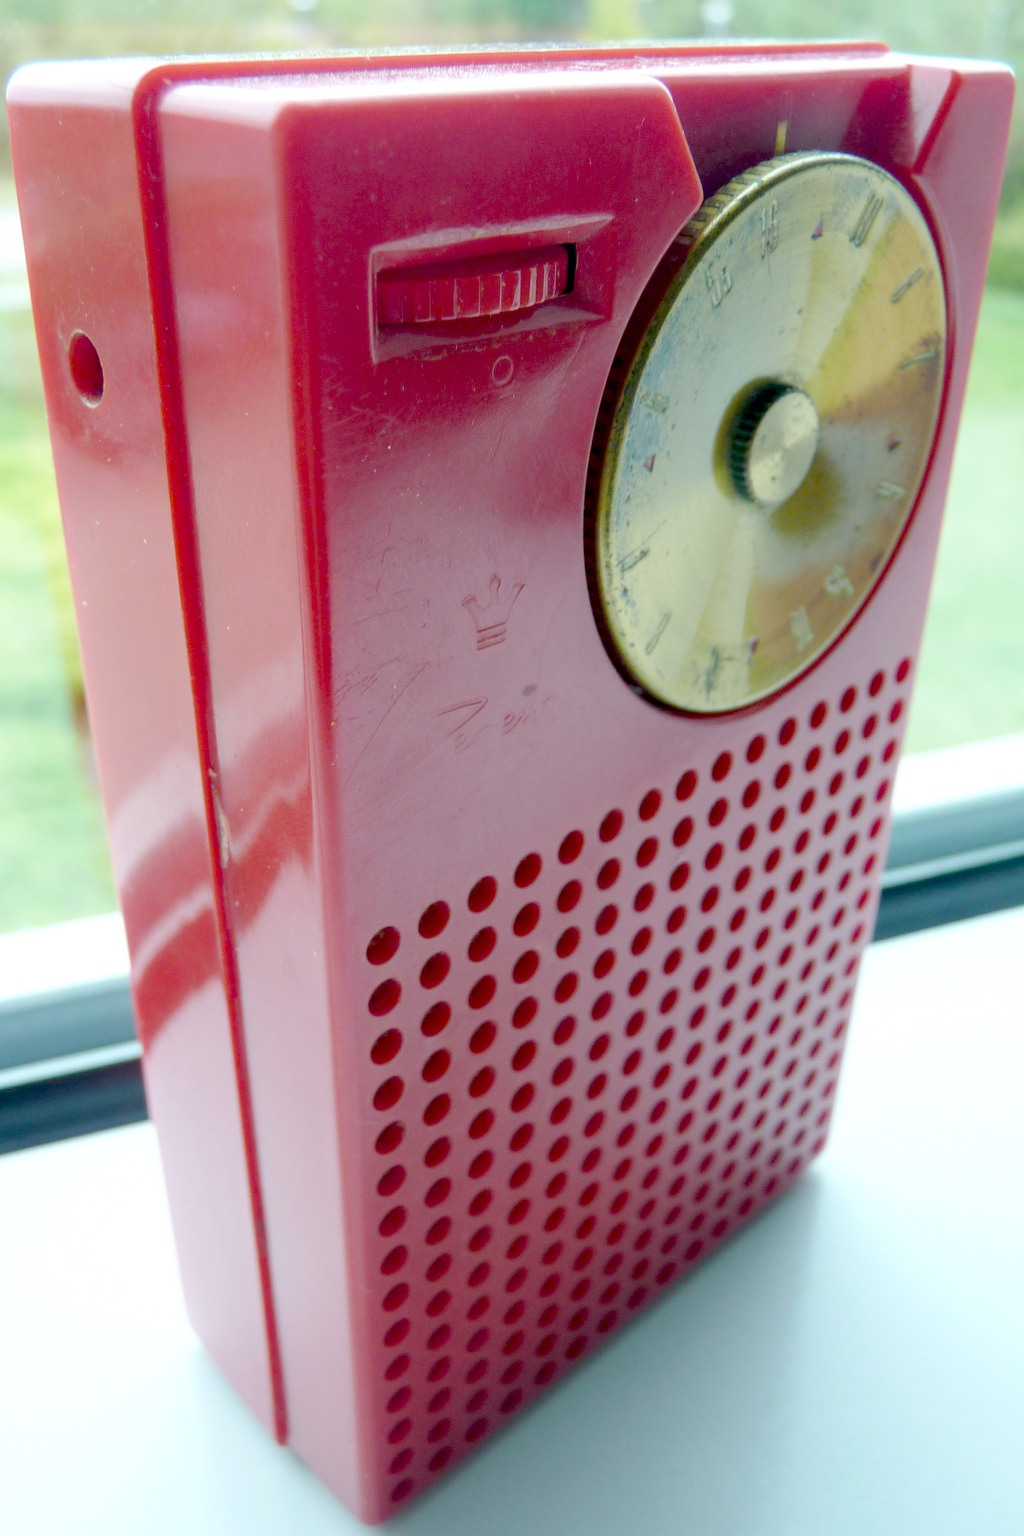
\includegraphics[scale = 0.2]{Graphics/Regency_TR-1_radio.jpg}
	\caption{radio \emph{Regency TR-1}.}
	\label{fig:4}
\end{figure}
\newpage

\section{La transición hacia un semiconductor más conveniente: El silicio}
El \textbf{germanio} era difícil de purificar y tenía un rango de temperatura operativa limitado. Los científicos tenían la teoría de que el \textbf{silicio}
sería más fácil de fabricar, pero pocos se molestaron en investigar esta posibilidad. \emph{Morris Tanenbaum} y algunos colaboradores en los \emph{Laboratorios Bell}
fueron los primeros en desarrollar un \textbf{transistor} de \textbf{silicio} funcional el 26 de enero de 1954. Unos meses más tarde, \emph{Gordon Teal}, trabajando
de forma independiente en \emph {Texas Instruments}, desarrolló un dispositivo similar.\\

\begin{figure}[htb]
	\centering
	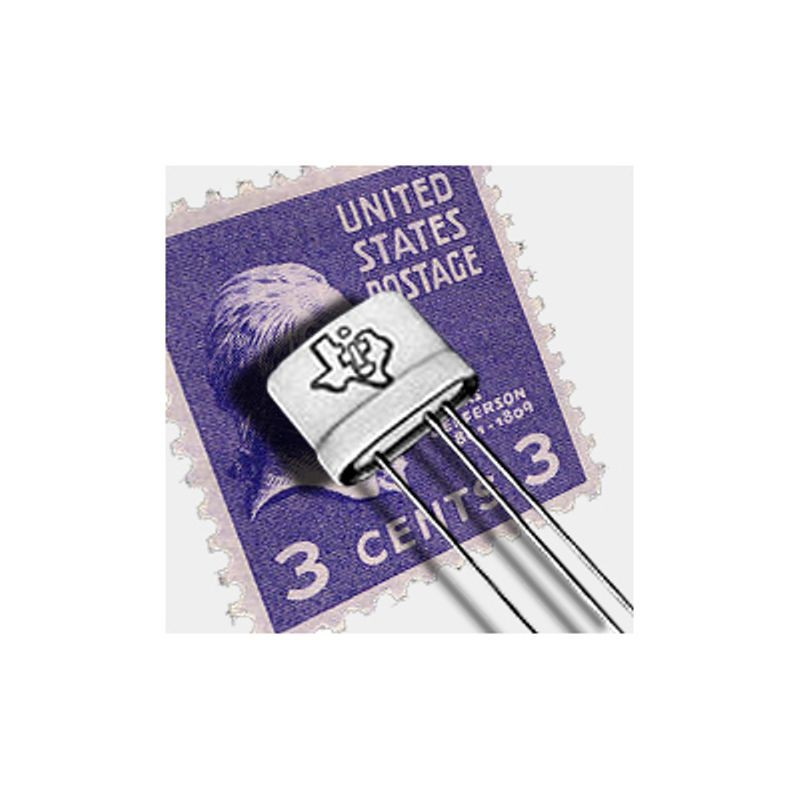
\includegraphics[scale = 0.2]{Graphics/texas_instruments_silicon_transistor.jpg}
	\caption{\textbf{transistor} de \textbf{silicio} de \emph{Texas Instruments}, anunciando su pequeño tamaño.}
	\label{fig:5}
\end{figure}

Ambos dispositivos se fabricaron controlando el dopaje de cristales de \textbf{silicio} individuales mientras crecían a partir de \textbf{silicio} fundido. \emph{Morris
Tanenbaum} y \emph{Calvin S. Fuller} desarrollaron un método superior en los \emph {Laboratorios Bell} a principios de 1955 mediante la difusión gaseosa de impurezas
donantes y aceptadoras en chips de \textbf{silicio} monocristalinos.\\
Sin embargo, hasta finales de la década de 1950, el \textbf{germanio} siguió siendo el material semiconductor dominante para los transistores y otros dispositivos
semiconductores. El \textbf{germanio} se consideró inicialmente el material semiconductor más eficaz, ya que podía demostrar un mejor rendimiento debido a una mayor
movilidad de los portadores. La relativa falta de rendimiento en los primeros semiconductores de \textbf{silicio} se debió a que la conductividad eléctrica estaba
limitada por estados superficiales cuánticos inestables, que impedían que la electricidad penetrara de manera confiable en la superficie para llegar a la capa de \textbf
{silicio} semiconductor.\\

\begin{figure}[htb]
	\centering
	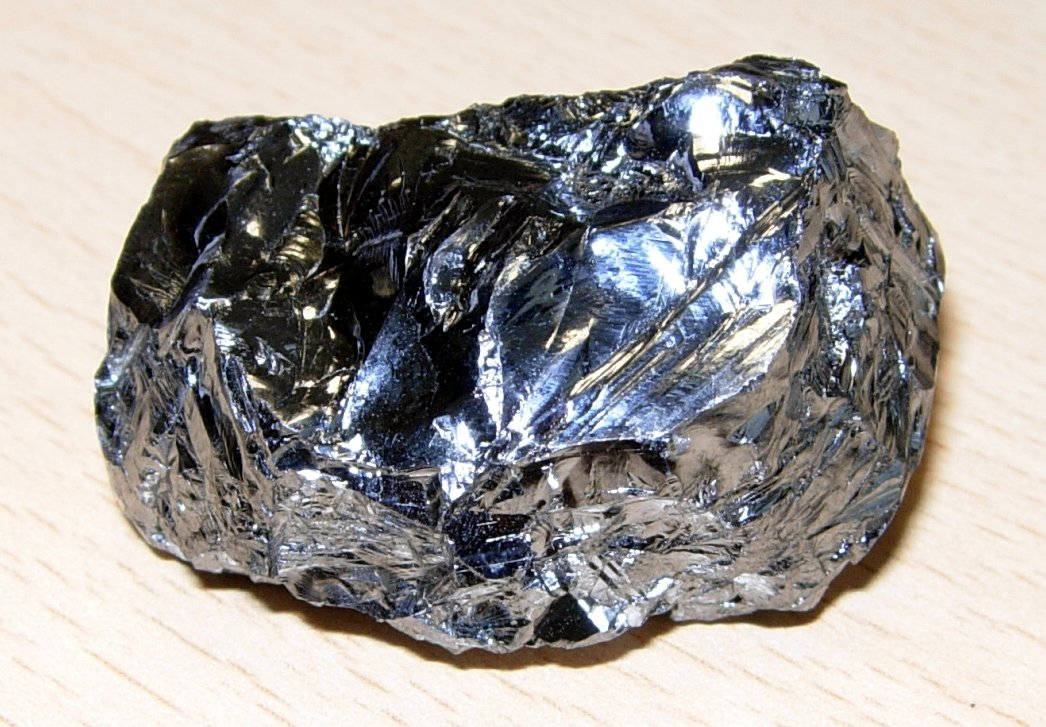
\includegraphics[scale = 0.2]{Graphics/silicon.jpg}
	\caption{Mineral de silicio}
	\label{fig:6}
\end{figure}

En 1955, \emph{Carl Frosch} y \emph{Lincoln Derick} de \emph{Bell Telephone Laboratories}(\textbf{BTL}) descubrieron accidentalmente que el dióxido de \textbf{silicio}(SiO2)
podía crecer sobre \textbf{silicio}. Demostraron que la capa de óxido evitaba que ciertos dopantes entraran en la oblea de \textbf{silicio}, mientras que permitía otros,
descubriendo así el \textbf{efecto pasivante} de la oxidación en la superficie del semiconductor. En la década de 1950, \emph{Mohamed Atalla}, retomó el trabajo de \emph{Frosch}
sobre la oxidación, investigó las propiedades superficiales de los semiconductores de \textbf{silicio} en los \emph{Laboratorios Bell}, donde propuso un nuevo método de fabricación
de dispositivos semiconductores, recubriendo una oblea de \textbf{silicio} con una capa aislante de óxido de \textbf{silicio} para que la electricidad podría penetrar de manera
confiable en el \textbf{silicio} conductor que se encuentra debajo, superando los estados superficiales que impedían que la electricidad llegara a la capa semiconductora. Esto
se conoce como \textbf{pasivación superficial}, un método que se volvió fundamental para la industria de los semiconductores, ya que más tarde hizo posible la producción en masa de
circuitos integrados de \textbf{silicio}.
